% Baccalauréat malgache, série C, 2006 : corrigé.
\TCDBacAttribution{C}{2006}
\providecommand{\cm}{~\mathrm{cm}}
\providecommand{\Plan}{(\mathscr{P})}
\providecommand{\dx}{~\mathrm{d}x}
\providecommand{\dt}{\mathrm{d}t}
\providecommand{\Ouv}{(O;\vec{u},\vec{v})}
\providecommand{\mes}[2]{\mathrm{mes}\left( \widehat{ \overrightarrow{#1} ; \overrightarrow{#2} } \right)}
\providecommand{\D}{(\mathscr{D})}
\providecommand{\Courbe}{(\mathscr{C})}
\providecommand{\Courben}{(\mathscr{C}_n)}
\providecommand{\CourbeU}{(\mathscr{C}_1)}
\providecommand{\CourbeD}{(\mathscr{C}_2)}
\providecommand{\bary}[1]{\mathrm{bar}\left\lbrace #1 \right\rbrace}
\providecommand{\congru}[3]{#1 \equiv #2 \quad \left[ \mathrm{mod}~#3\right]}
\providecommand{\Angl}[2]{\left( \widehat{ \overrightarrow{#1} , \overrightarrow{#2} } \right)}
%
\providecommand{\CourbeA}{(\mathscr{C}_\alpha)}
%%%%%%%%%%%%%%%%%%%%%%%%%%%%%%%%%%%%%%%%%%%%%%%%%%%%%%%%%%%%%%%%%%%%%%%%%%%%%%%%%%%%%%%%%%%%%%%%%%%%%%%%%%%%%%%%%%%%%%%%%%%%%%%%
\noindent \underline{\textsc{\textbf{Exercice}}} (4 points)
\begin{description}
	\item[I. ]
	\begin{enumerate}
		\item
		\begin{enumerate}
			\item \vln{Montrons que $n$ divise $8$ :}
				En base $n$ : $a = 2n^2 + n + 1$, $b = 3n^2 + n + 2$ et $c = n^5 + 3n^4 + 3n^3 + 0\cdot n^2 + 3n + 2$.
				En développant, $ab = 6n^4 + 5n^3 + 8n^2 + 3n + 2$. L'égalité $c = ab$ donne
				\[
					n^5 - 3n^4 - 2n^3 - 8n^2 = 0
					\iff n^2\left(n^3 - 3n^2 - 2n - 8\right) = 0 .
				\]
				Comme $n \neq 0$, on obtient $n^3 - 3n^2 - 2n = 8$, c'est-à-dire $n\left(n^2 - 3n - 2\right) = 8$ avec $n^2-3n-2$ entier.
				Donc \par\noindent\ansbox{$n$ divise $8$.}
			\item \vln{Valeur de $n$ :}
				Le chiffre $3$ figure dans l'écriture de $b$ et de $c$, donc $n \geq 4$. Les diviseurs de $8$ supérieurs ou égaux à $4$ sont $4$ et $8$.
				Pour $n = 4$ : $4^3 - 3\cdot 4^2 - 2\cdot 4 - 8 = 64 - 48 - 8 - 8 = 0$ ; pour $n = 8$ : $512 - 192 - 16 - 8 = 296 \neq 0$.
				Donc \par\noindent\ansbox{$n = 4$.}
			\item \vln{$a$ et $b$ en base dix :}
				$a = 2\cdot 16 + 4 + 1$ et $b = 3 \cdot 16 + 4 + 2$, donc \par\noindent\ansbox{$a = 37$ et $b = 54$.}
				(Vérification : $37 \times 54 = 1998$ et $c = 1024 + 3\cdot 256 + 3 \cdot 64 + 3\cdot 4 + 2 = 1998$.)
		\end{enumerate}
		\item \vln{Résolution de $37x + 54y = 3$ :}
			$\pgcd{37}{54} = 1$ divise $3$, donc l'équation a des solutions.
			On remarque que $37 \times 3 + 54 \times (-2) = 111 - 108 = 3$ : le couple $(3,-2)$ est une solution particulière.
			Si $(x,y)$ est solution, par soustraction $37(x-3) = -54(y+2) = 54(-2-y)$.
			Ainsi $54$ divise $37(x-3)$ et, comme $37$ et $54$ sont premiers entre eux, $54$ divise $x-3$ (théorème de Gauss) :
			$x = 3 + 54k$ avec $k \in \mathbb{Z}$, puis $37 \times 54 k = 54(-2-y)$, d'où $y = -2 - 37k$.
			Réciproquement ces couples conviennent : $37(3+54k) + 54(-2-37k) = 3$.
			\par\noindent\ansbox{$\mathcal{S} = \left\{ (3 + 54k \, ; \, -2 - 37k) \mid k \in \mathbb{Z} \right\}$.}
	\end{enumerate}
	\item[II. ]
	\begin{enumerate}
		\item \vln{Nombre de résultats possibles :}
			Un résultat est un rangement des quatre jetons, c'est-à-dire une permutation de $\{0,1,2,3\}$ :
			il y en a \par\noindent\ansbox{$4! = 24$.}
			Tous ces résultats sont équiprobables.
		\item
		\begin{itemize}
			\item \vln{Probabilité de $E$ :}
				Le troisième jeton est le $3$ ; les trois autres jetons occupent les trois autres places de $3! = 6$ façons.
				$P(E) = \frac{6}{24}$, soit \par\noindent\ansbox{$P(E) = \frac{1}{4}$.}
			\item \vln{Probabilité de $F$ :}
				Choisissons les trois numéros qui sortent en premier : $\Comb{4}{3} = 4$ choix.
				Parmi les $3! = 6$ ordres possibles de ces trois numéros, $F$ est réalisé exactement lorsque le plus petit et le plus grand
				sortent en premier et le numéro du milieu en troisième : $2$ ordres. Le dernier jeton est alors imposé.
				Donc $\mathrm{card}(F) = 4 \times 2 = 8$ et \par\noindent\ansbox{$P(F) = \frac{8}{24} = \frac{1}{3}$.}
			\item \vln{Probabilité de $G$ :}
				Le produit des deux derniers numéros est non nul si et seulement si aucun d'eux n'est $0$,
				c'est-à-dire si le jeton $0$ sort en première ou en deuxième position : $2 \times 3! = 12$ résultats.
				\par\noindent\ansbox{$P(G) = \frac{12}{24} = \frac{1}{2}$.}
		\end{itemize}
	\end{enumerate}
\end{description}
%%%%%%%%%%%%%%%%%%%%%%%%%%%%%%%%%%%%%%%%%%%%%%%%%%%%%%%%%%%%%%%%%%%%%%%%%%%%%%%%%%%%%%%%%%%%%%%%%%%%%%%%%%%%%%%%%%%%%%%%%%%%%%%%
\noindent \underline{\textsc{\textbf{PROBLEME I}}} (7 points) \newline
On a $AB = 2\cm$, $BC = 4\cm$ et, par Pythagore, $AC = \sqrt{16 - 4} = 2\sqrt{3}\cm$.
\begin{description}
	\item[Partie A :]
	\begin{enumerate}
		\item
		\begin{enumerate}
			\item \vln{Mesure de $\Angl{BA}{BC}$ :}
				Dans le triangle $ABC$ rectangle en $A$, $\cos \widehat{ABC} = \frac{AB}{BC} = \frac{1}{2}$, donc $\widehat{ABC} = \frac{\pi}{3}$.
				Comme $\mes{AB}{AC} = \frac{\pi}{2}$, le triangle $ABC$ est de sens direct ; l'angle orienté $\Angl{BA}{BC}$ est alors de sens indirect :
				\par\noindent\ansbox{$\mes{BA}{BC} = -\frac{\pi}{3}$.}
			\item \vln{Nature de $f = r_A \circ r_B$ :}
				On rappelle que si $D$ et $D'$ sont deux droites sécantes en $I$, $s_{D'} \circ s_D$ est la rotation de centre $I$ et d'angle $2\,(D , D')$.
				\begin{itemize}
					\item Soit $D_1$ la droite passant par $B$ telle que $\left(D_1 , (AB)\right) = \frac{\pi}{6}$ : alors $r_B = s_{(AB)} \circ s_{D_1}$.
					\item Soit $D_2$ la droite passant par $A$ telle que $\left((AB) , D_2\right) = \frac{\pi}{4}$ (bissectrice de l'angle droit $\widehat{BAC}$) : alors $r_A = s_{D_2} \circ s_{(AB)}$.
				\end{itemize}
				Donc $f = s_{D_2} \circ s_{(AB)} \circ s_{(AB)} \circ s_{D_1} = s_{D_2} \circ s_{D_1}$ car $s_{(AB)} \circ s_{(AB)} = \mathrm{Id}$.
				Les droites $D_1$ et $D_2$ ne sont pas parallèles ; elles se coupent en un point $\Omega$ et $2\,(D_1 , D_2) = 2\left(\frac{\pi}{6} + \frac{\pi}{4}\right) = \frac{5\pi}{6}$.
				\par\noindent\ansbox{$f$ est la rotation de centre $\Omega = D_1 \cap D_2$ et d'angle $\frac{5\pi}{6}$.}
		\end{enumerate}
		\item
		\begin{enumerate}
			\item \vln{Rapport et angle de $S$ :}
				$S(B) = B$ et $S(A) = C$, donc le rapport est $k = \frac{BC}{BA} = \frac{4}{2}$ et l'angle est $\Angl{BA}{BC}$ :
				\par\noindent\ansbox{$k = 2$ et $\theta = -\frac{\pi}{3}$.}
			\item \vln{Construction de $C_1 = S(C)$ :}
				La similitude $S$ conserve les angles ; elle transforme le triangle $BAC$, rectangle en $A$, en le triangle $BCC_1$, rectangle en $C$,
				avec $\Angl{BC}{BC_1} = -\frac{\pi}{3}$.
				Donc $C_1$ est le point d'intersection de la perpendiculaire à $(BC)$ en $C$ et de la demi-droite d'origine $B$ obtenue en tournant
				la demi-droite $[BC)$ de $-\frac{\pi}{3}$ (c'est le symétrique de la demi-droite $[BA)$ par rapport à $(BC)$).
				On a $BC_1 = 2 BC = 8\cm$.
				\begin{center}
				\begin{tikzpicture}[scale=.55,>=stealth]
					\coordinate (A) at (0,0); \coordinate (B) at (2,0); \coordinate (C) at (0,3.464);
					\coordinate (C1) at (6,6.928); \coordinate (C2) at (18,0);
					\draw[thin,gray] (-1,0) -- (19,0);
					\draw (A) -- (B) -- (C) -- cycle;
					\draw[blue] (B) -- (C1) -- (C);
					\draw[blue,dashed] (B) -- (C2) -- (C1);
					\draw[thin] (-1,2.887) -- (7,7.506);
					\foreach \P/\L/\pos in {A/A/below left,B/B/below,C/C/left,C1/C_1/above,C2/C_2/below} \fill (\P) circle (2pt) node[\pos] {$\L$};
				\end{tikzpicture}
				\end{center}
			\item \vln{Alignement de $A$, $B$, $C_2$ :}
				On a $C_2 = S(C_1) = S \circ S \circ S (A)$ ; $S\circ S\circ S$ est la similitude de centre $B$, de rapport $8$ et d'angle $3 \times \left(-\frac{\pi}{3}\right) = -\pi$.
				Donc $\Angl{BA}{BC_2} = -\pi \pmod{2\pi}$ : les vecteurs $\overrightarrow{BA}$ et $\overrightarrow{BC_2}$ sont colinéaires (de sens contraires), et
				\par\noindent\ansbox{$A$, $B$ et $C_2$ sont alignés ($\overrightarrow{BC_2} = -8\,\overrightarrow{BA}$).}
		\end{enumerate}
	\end{enumerate}
	\item[Partie B :]
	\begin{enumerate}
		\item \vln{Affixes :}
			$\overrightarrow{AB} = 2\vec{u}$ et $\overrightarrow{AC} = 2\sqrt{3}\,\vec{v}$, donc \par\noindent\ansbox{$z_A = 0$, $z_B = 2$, $z_C = 2\sqrt{3}\, i$.}
		\item
		\begin{enumerate}
			\item \vln{Expressions complexes :}
				$r_A : z' = \expo{i\frac{\pi}{2}} z$, soit \par\noindent\ansbox{$r_A : z' = iz$.}
				$r_B : z' - 2 = \expo{i\frac{\pi}{3}} (z - 2)$, soit \par\noindent\ansbox{$r_B : z' = \left(\tfrac{1}{2} + i\tfrac{\sqrt{3}}{2}\right) z + 1 - i\sqrt{3}$.}
				Alors $f(z) = i\left[\left(\tfrac{1}{2} + i\tfrac{\sqrt{3}}{2}\right) z + 1 - i\sqrt{3}\right]$, d'où
				\par\noindent\ansbox{$f : z' = \left(-\tfrac{\sqrt{3}}{2} + \tfrac{1}{2} i\right) z + \sqrt{3} + i$.}
			\item \vln{Éléments caractéristiques de $f$ :}
				$-\frac{\sqrt{3}}{2} + \frac{1}{2} i = \expo{i\frac{5\pi}{6}}$ est de module $1$ et différent de $1$ : $f$ est une rotation d'angle $\frac{5\pi}{6}$.
				Son centre $\Omega$ vérifie $\omega = \expo{i\frac{5\pi}{6}}\omega + \sqrt{3} + i$, d'où
				\[
					\begin{aligned}
					\omega &= \frac{\sqrt{3} + i}{1 + \frac{\sqrt{3}}{2} - \frac{1}{2}i}
						= \frac{2(\sqrt{3}+i)}{(2+\sqrt{3}) - i}
						= \frac{2(\sqrt{3}+i)\left((2+\sqrt{3}) + i\right)}{(2+\sqrt{3})^2 + 1} \\
						&= \frac{2\left[(2\sqrt{3}+2) + (2\sqrt{3}+2) i\right]}{8 + 4\sqrt{3}}
						= \frac{(\sqrt{3}+1)(1+i)}{2+\sqrt{3}} .\end{aligned}
				\]
				Comme $\frac{\sqrt{3}+1}{2+\sqrt{3}} = (\sqrt{3}+1)(2-\sqrt{3}) = \sqrt{3} - 1$ :
				\par\noindent\ansbox{$f$ est la rotation de centre $\Omega\left(\sqrt{3}-1 \, ; \, \sqrt{3}-1\right)$ et d'angle $\frac{5\pi}{6}$.}
				On retrouve la partie A : $\Omega$ est sur la droite $D_2$ d'équation $y = x$ et sur la droite $D_1$ d'équation $y = -\frac{1}{\sqrt{3}}(x-2)$.
		\end{enumerate}
		\item \vln{Expression complexe de $S$ :}
			$S$ a pour forme $z' = az + b$ avec $S(B) = B$ et $S(A) = C$ : $2 = 2a + b$ et $2\sqrt{3}\,i = b$, d'où $a = 1 - i\sqrt{3}$.
			\par\noindent\ansbox{$S : z' = \left(1 - i\sqrt{3}\right) z + 2\sqrt{3}\, i$.}
			Comme $1 - i\sqrt{3} = 2\expo{-i\frac{\pi}{3}}$, $S$ est la similitude directe de centre $B$ (le point invariant : $\frac{2\sqrt{3}i}{1 - (1-i\sqrt{3})} = 2$),
			de rapport $2$ et d'angle $-\frac{\pi}{3}$, ce qui confirme la partie A.
			(On trouve aussi $z_{C_1} = 6 + 4\sqrt{3}\, i$ et $z_{C_2} = 18$, réel : $C_2 \in (AB)$.)
		\item
		\begin{enumerate}
			\item \vln{Images de $B$ et $C$ :}
				$g(2) = 2\left(-1 - i\sqrt{3}\right) + 4 + 2i\sqrt{3} = 2$ ;
				$g(2\sqrt{3}\,i) = \left(-1 - i\sqrt{3}\right)\left(-2\sqrt{3}\, i\right) + 4 + 2i\sqrt{3} $ \\ $\phantom{g(2\sqrt{3}\,i)} = 2\sqrt{3}\, i - 6 + 4 + 2i\sqrt{3}$.
				\par\noindent\ansbox{$z_{B'} = 2$ (donc $B' = B$) et $z_{C'} = -2 + 4\sqrt{3}\, i$.}
			\item \vln{Alignement de $B$, $C$, $C'$ :}
				$z_{C'} - z_B = -4 + 4\sqrt{3}\, i = 2\left(-2 + 2\sqrt{3}\, i\right) = 2\left(z_C - z_B\right)$.
				\par\noindent\ansbox{$\overrightarrow{BC'} = 2\, \overrightarrow{BC}$ : $B$, $C$, $C'$ sont alignés.}
			\item \vln{Éléments caractéristiques de $g$ :}
				$g$ est de la forme $z' = a\bar{z} + b$ avec $|a| = \left|-1 - i\sqrt{3}\right| = 2 \neq 0$ : c'est une similitude indirecte de rapport $2$.
				Comme le rapport est différent de $1$, elle a un unique point fixe, qui est $B$ d'après (a).
				Soit $h$ l'homothétie de centre $B$ et de rapport $2$ ; alors $s = g \circ h^{-1}$ est une similitude indirecte de rapport $1$ qui fixe $B$
				et aussi $C'$ car $h^{-1}(C') = C$ et $g(C) = C'$. Une isométrie indirecte fixant deux points distincts est la symétrie orthogonale d'axe la droite qui les joint :
				$s = s_{(BC)}$ et $g = s_{(BC)} \circ h$.
				\par\noindent\ansbox{$g$ est la similitude indirecte de centre $B$, de rapport $2$ et d'axe $(BC)$.}
		\end{enumerate}
	\end{enumerate}
\end{description}
%%%%%%%%%%%%%%%%%%%%%%%%%%%%%%%%%%%%%%%%%%%%%%%%%%%%%%%%%%%%%%%%%%%%%%%%%%%%%%%%%%%%%%%%%%%%%%%%%%%%%%%%%%%%%%%%%%%%%%%%%%%%%%%%
\noindent \underline{\textsc{\textbf{PROBLEME II}}} (9 points)
\begin{description}
	\item[Partie A]
	\begin{enumerate}
		\item \vln{Sens de variation de $f_\alpha$ suivant le signe de $\alpha$ :}
			Pour $x > 0$, $f_\alpha$ est dérivable et
			$f_\alpha'(x) = \alpha x^{\alpha-1}\expo{1-x} - x^\alpha \expo{1-x} = x^{\alpha - 1}\expo{1-x}\,(\alpha - x)$.
			Comme $x^{\alpha-1}\expo{1-x} > 0$, $f_\alpha'(x)$ a le signe de $\alpha - x$.
			\begin{itemize}
				\item Si $\alpha < 0$ : $\alpha - x < 0$ pour tout $x > 0$, donc \par\noindent\ansbox{$f_\alpha$ est strictement décroissante sur $]0 ; +\infty[$.}
					(Dans ce cas $\lim_{x\to 0^+} x^\alpha = +\infty$ : $f_\alpha$ n'est pas continue en $0$, où elle vaut $0$ par définition.)
				\item Si $\alpha > 0$ : \par\noindent\ansbox{$f_\alpha$ est croissante sur $[0 ; \alpha]$ et décroissante sur $[\alpha ; +\infty[$,}
					avec un maximum $f_\alpha(\alpha) = \alpha^\alpha \expo{1-\alpha}$. Ici $\lim_{x\to 0^+} x^\alpha = 0$ : $f_\alpha$ est continue en $0$.
			\end{itemize}
		\item
		\begin{enumerate}
			\item \vln{Tableau de variation de $f_1$ :}
				$f_1(x) = x\expo{1-x}$, $f_1'(x) = (1-x)\expo{1-x}$, $f_1(1) = 1$.
				En $+\infty$ : $f_1(x) = e \cdot \frac{x}{\expo{x}}$ et $\lim_{x\to+\infty} \frac{x}{\expo{x}} = 0$, donc $\lim_{x\to+\infty} f_1(x) = 0$.
				\[
				\begin{array}{c|ccccc}
					x & 0 & & 1 & & +\infty \\ \hline
					f_1'(x) & e & + & 0 & - & \\ \hline
					 & & & 1 & & \\
					f_1 & & \nearrow & & \searrow & \\
					 & 0 & & & & 0
				\end{array}
				\]
			\item \vln{Courbe $\CourbeU$ :}
				Éléments utiles : la droite $y = 0$ est asymptote en $+\infty$ ; la tangente à l'origine a pour équation $y = ex$ ($f_1'(0) = e$) ;
				la tangente au point $(1 ; 1)$ est horizontale ; $f_1''(x) = (x-2)\expo{1-x}$ s'annule en changeant de signe en $2$ :
				point d'inflexion $\left(2 ; \frac{2}{e}\right) \approx (2 ; 0{,}74)$.
				\begin{center}
				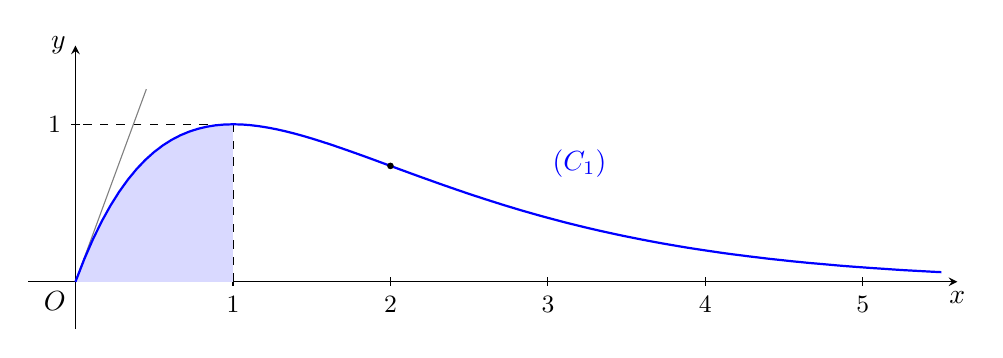
\begin{tikzpicture}[x=2cm,y=2cm,>=stealth]
					\draw[->] (-0.3,0) -- (5.6,0) node[below] {$x$};
					\draw[->] (0,-0.3) -- (0,1.5) node[left] {$y$};
					\foreach \t in {1,2,3,4,5} \draw (\t,0.03) -- (\t,-0.03) node[below] {\small $\t$};
					\draw (0.03,1) -- (-0.03,1) node[left] {\small $1$};
					\node[below left] at (0,0) {$O$};
					\draw[dashed] (1,0) -- (1,1) -- (0,1);
					\draw[gray] (0,0) -- (0.45,1.223);
					\fill[blue!15] (0,0) -- plot[domain=0:1,samples=40] (\x,{\x*exp(1-\x)}) -- (1,0) -- cycle;
					\draw[blue,thick] plot[domain=0:5.5,samples=100] (\x,{\x*exp(1-\x)});
					\fill (2,0.7358) circle (1.2pt);
					\node[blue] at (3.2,0.75) {$\CourbeU$};
				\end{tikzpicture}
				\end{center}
			\item \vln{Calcul de $I$ :}
				Posons $u(x) = x$, $v'(x) = \expo{1-x}$ ; $u'(x) = 1$, $v(x) = -\expo{1-x}$.
				\[
					\int_0^1 x\expo{1-x}\dx = \left[-x\expo{1-x}\right]_0^1 + \int_0^1 \expo{1-x}\dx = -1 + \left[-\expo{1-x}\right]_0^1 = -1 - 1 + e = e - 2 .
				\]
				Donc \par\noindent\ansbox{$I = 4(e-2) = 4e - 8 \approx 2{,}87$.}
				Interprétation : $f_1 \geq 0$ sur $[0;1]$, donc $\int_0^1 f_1(x)\dx$ est l'aire, en unités d'aire, du domaine limité par $\CourbeU$, l'axe des abscisses
				et les droites $x = 0$, $x = 1$ (domaine colorié). L'unité d'aire vaut $2\cm \times 2\cm = 4\,\mathrm{cm}^2$ :
				\par\noindent\ansbox{$I$ est l'aire de ce domaine exprimée en $\mathrm{cm}^2$, soit environ $2{,}87\,\mathrm{cm}^2$.}
		\end{enumerate}
		\item
		\begin{enumerate}
			\item \vln{$f_1$ est solution de $(E)$ :}
				$f_1'(x) = (1-x)\expo{1-x}$ et $f_1''(x) = -\expo{1-x} - (1-x)\expo{1-x} = (x-2)\expo{1-x}$. Alors
				\[
					f_1'' - 2f_1' + f_1 = \left[(x - 2) - 2(1-x) + x\right]\expo{1-x} = (4x - 4)\expo{1-x} = 4(x-1)\expo{1-x} .
				\]
				\par\noindent\ansbox{$f_1$ est bien une solution de $(E)$.}
			\item \vln{Résolution de $(E')$ puis de $(E)$ :}
				L'équation caractéristique $r^2 - 2r + 1 = 0$, soit $(r-1)^2 = 0$, a la racine double $r = 1$.
				\par\noindent\ansbox{Les solutions de $(E')$ sont $y = (Ax + B)\expo{x}$, $A, B \in \mathbb{R}$.}
				Une fonction $y$ est solution de $(E)$ si et seulement si $y - f_1$ est solution de $(E')$ (l'équation est linéaire). Donc
				\par\noindent\ansbox{Les solutions de $(E)$ sont $y = (Ax+B)\expo{x} + x\expo{1-x}$, $A, B \in \mathbb{R}$.}
		\end{enumerate}
	\end{enumerate}
	\item[Partie B]
	\begin{enumerate}
		\item
		\begin{enumerate}
			\item \vln{Encadrement de $I_n$ :}
				Pour $0 \leq x \leq 1$, $0 \leq 1 - x \leq 1$, donc, l'exponentielle étant croissante, $1 \leq \expo{1-x} \leq e$.
				En multipliant par $x^n \geq 0$ : $x^n \leq x^n \expo{1-x} \leq e\,x^n$. On intègre sur $[0;1]$ (bornes dans l'ordre croissant) :
				\[
					\int_0^1 x^n \dx \leq I_n \leq e\int_0^1 x^n \dx
					\quad\text{avec}\quad \int_0^1 x^n\dx = \frac{1}{n+1} .
				\]
				\par\noindent\ansbox{$\frac{1}{n+1} \leq I_n \leq \frac{e}{n+1}$.}
			\item \vln{Relation de récurrence :}
				Posons $u(x) = x^{n+1}$, $v'(x) = \expo{1-x}$ ; $u'(x) = (n+1)x^n$, $v(x) = -\expo{1-x}$ :
				\[
					I_{n+1} = \left[-x^{n+1}\expo{1-x}\right]_0^1 + (n+1)\int_0^1 x^n\expo{1-x}\dx = -1 + (n+1) I_n .
				\]
				\par\noindent\ansbox{$I_{n+1} = (n+1) I_n - 1$.}
		\end{enumerate}
		\item
		\begin{enumerate}
			\item \vln{Calcul de $J_1$ :}
				$I_1 = \int_0^1 x \expo{1-x}\dx = e - 2$ (partie A), donc $J_1 = 1!\, e - (e-2)$ : \par\noindent\ansbox{$J_1 = 2$.}
			\item \vln{Relation entre $J_{n+1}$ et $J_n$ :}
				$J_{n+1} = (n+1)!\, e - I_{n+1} = (n+1)\, n!\, e - (n+1) I_n + 1 = (n+1)\left(n!\, e - I_n\right) + 1$.
				\par\noindent\ansbox{$J_{n+1} = (n+1) J_n + 1$.}
				Récurrence : $J_1 = 2$ est un entier naturel ; si $J_n$ est un entier naturel, alors $(n+1)J_n + 1$ en est un aussi.
				\par\noindent\ansbox{Pour tout $n \geq 1$, $J_n$ est un entier naturel.}
			\item \vln{$n!\, e$ n'est pas entier pour $n \geq 2$ :}
				Pour $n \geq 2$, d'après 1.(a), $0 < \frac{1}{n+1} \leq I_n \leq \frac{e}{n+1} \leq \frac{e}{3} < 1$.
				Donc $J_n < n!\, e = J_n + I_n < J_n + 1$ : le nombre $n!\, e$ est strictement compris entre deux entiers consécutifs.
				\par\noindent\ansbox{Pour $n \geq 2$, $n!\, e$ n'est pas un entier naturel.}
			\item \vln{Irrationalité de $e$ :}
				Si $n \geq q$, alors $q$ est l'un des facteurs de $n! = 1 \times 2 \times \cdots \times n$, donc $\frac{n!}{q}$ est un entier naturel et
				$n!\,\frac{p}{q} = p \times \frac{n!}{q}$ est un entier naturel.

				Supposons $e = \frac{p}{q}$ avec $p, q$ entiers naturels non nuls ($e > 0$). Prenons $n \geq \max(q, 2)$ :
				$n!\, e = n!\, \frac{p}{q}$ serait un entier naturel, ce qui contredit (c).
				\par\noindent\ansbox{$e$ n'est pas un nombre rationnel.}
		\end{enumerate}
	\end{enumerate}
\end{description}
